\section{Performance-Analyse}
Selbstverständlich ist für eine richtige Implementierung nicht nur wichtig, dass diese funktioniert. Sie muss dies auch möglichst performant und effizient tun. Hierzu werden mehrere Testläufe in Hinblick auf die Performance durchgeführt. Im Folgenden werden diese Testfälle beschrieben, sowie auch die Hardware, auf welcher die Tests durchgeführt werden. Ohne die Referenz zur verwendeten Hardware wäre eine Aussage über die Performance nur sehr bedingt verwendbar. In Abbildung \ref{hardware} sind die relevanten Komponenten aufgelistet. Zu beachten ist hierbei, dass AMD-Prozessoren allgemein eine höhere Multithreading-Performance besitzen, welche in der vorliegenden Software genutzt wird.
\begin{table}[H]
	\centering
	\setstretch{0.75}
	\begin{tabular}{c c c c c c c}
		Komponente & Name & Technische Daten\\
		CPU & AMD FX8350 & 8 Kerne, 4.2 GHz\\ 
		RAM & Kingston 99U5471 & 24 GB DDR3, 666 MHz  \\ 
	\end{tabular}
	\caption{Für Performance-Benchmarks verwendete relevante Hardware}
	\label{hardware}
\end{table}
Als Grundlage der Benchmarks wird das a280-\ac{TSP} verwendet um zum Einen eine standardisierte Grundlage zu erhalten und zum Anderen um eine genügend große Problemstellung zu erzeugen, die bezogen auf den Rechenaufwand auch relevant ist. Es wurden 8 parallele Threads gestartet, um eine hohe Auslastung der Hardware zu gewährleisten, ohne durch zu umfangreiches Threadhandling Performance einzubüßen. Die Applikation wurde genau 60 Sekunden lang betrieben, um einen einfachen Vergleichswert zu erhalten.

\newpage
\subsection{CPU-Auslastung}
Wie in Abbildung \ref{cpuUsage} zu sehen ist, beansprucht die Applikation durchgehend zwischen 60 und 70 Prozent. Dass keine 100 Prozent genutzt werden können, liegt daran, dass die Test-Umgebung nicht optimal ist. So wurden die Benchmarks auf einem Desktop-PC in normalen Betrieb mit gleichzeitiger Heim-Nutzung durchgeführt. Da für das Betriebssystem keine Priorisierung der Applikation vorliegt, wird diese mit anderen Programmen gleichgestellt und die Ressourcen auch dementsprechend verteilt.

\begin{figure}[h]
	\centering
	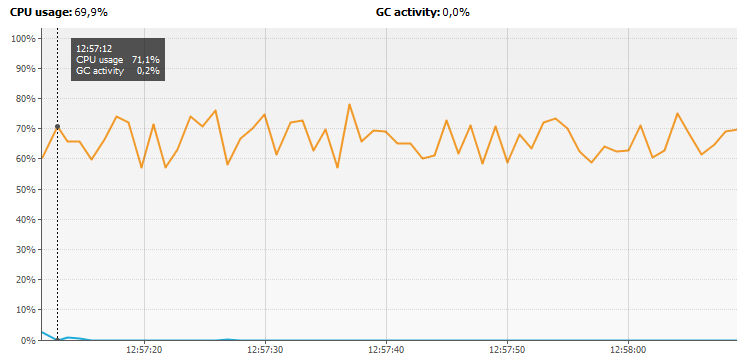
\includegraphics[width=0.9\linewidth]{images/cpuUsage.png}
	\caption{Aufzeichnung der CPU-Beanspruchung der Applikation über die gesamte Laufzeit}
	\label{cpuUsage}
\end{figure}

Würde die Applikation auf einer einwandfreien Test-Umgebung betrieben werden, würden bis zu 100 Prozent der CPU genutzt werden, was zu einer Verbesserung der Performance führen würde. Aber eine hohe Nutzung der CPU alleine kann nicht beschreiben, wie effizient ein Programm arbeitet. Hierzu sind noch andere Parameter notwendig, wie zum Beispiel die Nutzung des Hauptspeichers.

\subsection{Heap-Nutzung}
In Abbildung \ref{heapUsage} ist eine Statistik des benötigten Heaps der Applikation über die Laufzeit zu sehen. In blau markiert ist der benötigte Speicher im Heap zu einem bestimmten Zeitpunkt. In orange hinterlegt ist die Menge an Speicher, welche vom Programm allokiert wurde. Es lassen sich hierbei mehrere Aussagen ableiten. 

Zum Einen ist die Speicherallokierung konstant. Es werden vom Programm immer 2,4 GB an RAM belegt. Zum Anderen ist der Unterschied zwischen belegtem und allokierten Speicher teilweise enorm, was aber nicht auf die Arbeitsweise des Programms zurückzuführen ist. Zusätzlich lässt sich über die Grafik auch noch bestätigen, dass der GarbageCollector von Java zuverlässig nicht mehr benötigte Strukturen im Heap wieder frei gibt, was durch die lokalen Tiefpunkte im Heap-Verbrauch ersichtlich wird.

\begin{figure}[h]
	\centering
	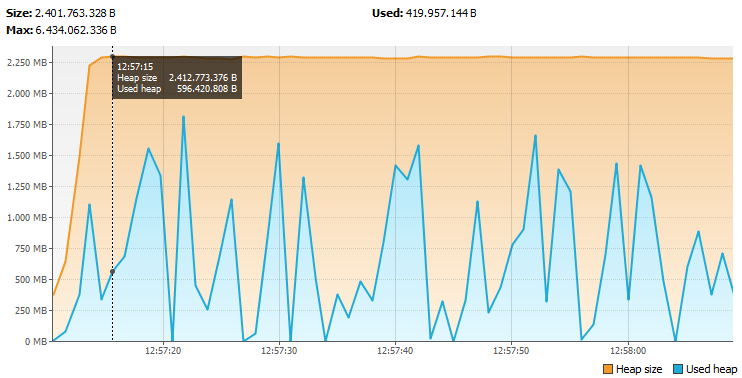
\includegraphics[width=0.9\linewidth]{images/heapUsage.png}
	\caption{Aufzeichnung des Speicherverbrauchs der Applikation über die gesamte Laufzeit. Blau markiert ist der derzeit verwendete Speicher, in orange der allokierte Speicher.}
	\label{heapUsage}
\end{figure}

Als möglichen Optimierungspunkt lässt sich hier der überdimensionierte Heap nennen. Mit 2,4 GB ist der Verbrauch zwar nicht so hoch, dass er eine Verwendung auf einer heutigen Hardware verhindert. Allerdings ist bei einem Anspruch einer möglichst effizienten Software dieser unnötige Verbrauch nicht haltbar.

\subsection{Anzahl Threads pro Minute}
Schlussendlich ist nicht die Auslastung der Hardware ausschlaggebend für die Performance eines Algorithmus, sondern wie effizient dieser rechnet. Als Richtwert kann in diesem Beispiel die Anzahl an Threads pro Minute herangezogen werden, da ein Thread einem Rechenschritt entspricht bzw. über die Anzahl an Threads auch die Anzahl an Generationen errechnet werden können. Die Anzahl an Generationen ist hierbei ein direkter Richtwert wie viele Routen abgelaufen werden konnten.

In Abbildung \ref{threadUsage} ist eine Statistik der in der Applikation aktiven Threads aufgezeigt. In blau werden die Daemon-Threads - hauptsächlich Systemthreads, wie beispielsweise der GarbageCollector - und in rot die Live-Threads gezeigt. Die Menge an aktiven Live-Threads beläuft sich im Durchschnitt auf 19. Für die Berechnung werden pro Generation acht Threads gestartet, welche nach der Generation auch wieder abgebaut werden. Somit ist auch hier wieder ein Overhead vom System vorhanden - in Summe 11 Live-Threads und 10 Daemon-Threads.

\begin{figure}[h]
	\centering
	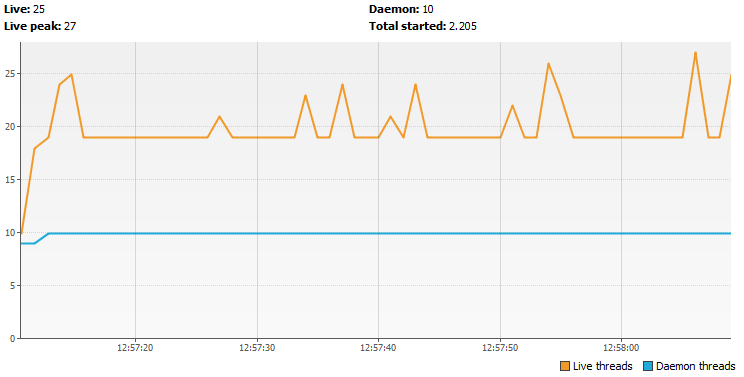
\includegraphics[width=0.9\linewidth]{images/threadUsage.png}
	\caption{Aufzeichnung der Menge an gleichzeitig aktiven Threads des Programms. In blau gezeichnet ist die Menge an Daemon-Threads, in orange die Anzahl an aktiven Live-Threads.}
	\label{threadUsage}
\end{figure}

Mithilfe der Datenerfassung lässt sich auch die genaue Anzahl an gestarteten Threads innerhalb der Applikation ermitteln. Innerhalb von 60 Sekunden wurden 2170 Threads bzw. Ameisen gestartet. Somit wurden ca 36,1 Ameisen pro Sekunde generiert. Teilt man diese Menge durch die Anzahl an Ameisen pro Generation (also acht) erhält man die Menge an Generationen pro Sekunde - in diesem Fall ca. 4,5.

\newpage
\subsection{Fazit zur Performance}
Nun wurden im Detail die relevanten Daten zur Performance genannt und analysiert. Als Fazit können einige Punkte genannt werden:
\begin{itemize}
	\item Die CPU wird fast vollständig genutzt
	\item Der Heap-Verbrauch ist akzeptabel, aber nicht optimal
	\item Es werden bei acht gleichzeitigen Ameisen 4,5 Generationen des a280-Problem pro Sekunde berechnet
\end{itemize}
Diese Aussagen ergeben eine relativ gute Bewertung der Applikation in Hinblick auf die Performance. Allerdings wurden bereits Schwachstellen erkannt. So ist die Belegung des Speichers im Vergleich zum wirklichen Verbrauch teilweise sehr hoch. Auch entsteht durch System-Threads ein recht großer Overhead. Im weiteren Entwicklungsverlauf dieser Applikation sollte in diesen Punkten noch eine Optimierung vorgenommen werden.